%==============================================================================
% QSD SUPPLEMENT S5: SYNDROME PREDICTION AND PROTON STABILITY
% LHC Phenomenology, Proton Decay, and Falsification Criteria
%==============================================================================

\documentclass[11pt,a4paper]{article}

\usepackage[utf8]{inputenc}
\usepackage[T1]{fontenc}
\usepackage{amsmath,amssymb,amsthm,mathtools}
\usepackage{geometry}
\usepackage{booktabs}
\usepackage{array}
\usepackage{xcolor}
\usepackage{physics}
\usepackage{hyperref}
\usepackage{enumitem}
\usepackage{float}
\usepackage{tikz}
\usetikzlibrary{shapes,arrows.meta,positioning,calc,decorations.text,decorations.pathmorphing,decorations.markings,decorations.pathreplacing}
\usepackage{orcidlink}
\usepackage{hyperref}
\hypersetup{colorlinks=true, linkcolor=blue, citecolor=blue, urlcolor=blue}

\geometry{margin=1in}

\hypersetup{
    colorlinks=true,
    linkcolor=blue!70!black,
    citecolor=blue!70!black,
    urlcolor=blue!70!black
}

% Theorem environments
\newtheorem{theorem}{Theorem}[section]
\newtheorem{lemma}[theorem]{Lemma}
\newtheorem{proposition}[theorem]{Proposition}
\newtheorem{corollary}[theorem]{Corollary}
\theoremstyle{definition}
\newtheorem{definition}[theorem]{Definition}
\theoremstyle{remark}
\newtheorem{remark}[theorem]{Remark}

% ---- QSD Notation (Hb convention, matching S1--S4) ----
\newcommand{\Hb}{\textnormal{H\kern-0.3em b}}
\newcommand{\Hbn}{\Hb_n}
\newcommand{\Hbfour}{\Hb_4}
\newcommand{\strain}{\varsigma}            % Graph strain (C₅-route value adopted)
\newcommand{\gr}{\varphi}
\newcommand{\murad}{\mu_0}
\newcommand{\nurad}{\nu_0}
\newcommand{\Mpl}{M_{\mathrm{Pl}}}
\newcommand{\MX}{{M_X^{\mathrm{QSD}}}}
\newcommand{\mH}{m_H}
\newcommand{\Esyn}{E_{\mathrm{syn}}}
\newcommand{\Psyn}{P_{\mathrm{syn}}}
\newcommand{\Punc}{P_{\mathrm{unc}}}
\newcommand{\aem}{\alpha_{\mathrm{em}}}
\newcommand{\tW}{\theta_W}
\newcommand{\LL}{\mathcal{L}}

% Colors
\definecolor{bulkcolor}{RGB}{70,130,180}
\definecolor{anchorcolor}{RGB}{200,40,40}
\definecolor{goldenphi}{RGB}{180,140,40}
\definecolor{syndromecolor}{RGB}{220,120,30}
\definecolor{straincolor}{RGB}{40,160,80}
\definecolor{protoncolor}{RGB}{100,50,180}
\definecolor{falsifycolor}{RGB}{180,30,30}

\title{
  \textbf{QSD Supplement S5: \\[0.5em] Syndrome Prediction and Proton Stability}\\[0.5em]
  \Large LHC Phenomenology, Proton Decay, and Falsification Criteria\\[1em]
}

\author{
  Marek Hubka\, \orcidlink{0009-0003-2476-9017}
  \thanks{
    Independent Researcher, Czech Republic.\\
    Website: \href{http://www.tidesofuncertainty.com}{tidesofuncertainty.com}.\\
    Email: \href{mailto:marek@tidesofuncertainty.com}{marek@tidesofuncertainty.com}.
  }
}

\date{\today}

\begin{document}

\maketitle

\begin{abstract}
\noindent This supplement derives the two most directly testable predictions of Quantum Spectrodynamics: the syndrome energy $\Esyn = 28.24$~GeV observable at the LHC, and the proton lifetime $\tau_p \sim 10^{39}$~years testable at Hyper-Kamiokande. The syndrome energy is derived from the anchor binding energy released during the ``Snap'' mechanism, with binding contributions from 4 severed bonds each contributing $2\strain$ of strain energy. The mass-proportional radion coupling determines branching ratios: $\mathrm{BR}(b\bar{b}) = 83.6\%$, $\mathrm{BR}(\tau^+\tau^-) = 5.6\%$, $\mathrm{BR}(\mu^+\mu^-) = 0.020\%$. We explain the 8~TeV vs.\ 13~TeV significance puzzle through strain-budget dilution, prove that the syndrome signal saturates rather than growing with luminosity, and derive proton stability from the QSD grand unification scale $\MX = \Mpl\strain = 1.75 \times 10^{17}$~GeV, yielding $\tau_p \approx 2 \times 10^{39}$~years via standard dimensional scaling. Sharp falsification criteria are established for LHC Run~3 and next-generation proton decay experiments.
\end{abstract}

\tableofcontents
\newpage

%==============================================================================
\section{The Syndrome Concept}
\label{sec:concept}
%==============================================================================

\subsection{Error Correction and Syndromes}

In quantum error correction, a \textbf{syndrome} is the measurement outcome~\cite{NielsenChuang2010,Gottesman1997} that reveals which error occurred on a codeblock, without revealing the encoded logical information. Syndromes are central to fault-tolerant quantum computation: they allow errors to be diagnosed and corrected without destroying the protected qubit.

\begin{definition}[Syndrome in QEC]
For a stabilizer code with generators $\{g_1, \ldots, g_k\}$, the syndrome of an error $E$ is the binary vector:
\begin{equation}
\mathbf{s}(E) = (s_1, \ldots, s_k), \quad s_i = \begin{cases} 0 & \text{if } [E, g_i] = 0 \\ 1 & \text{if } \{E, g_i\} = 0 \end{cases}
\end{equation}
\end{definition}

For the $[[5,1,3]]$ code, there are 4 stabilizer generators and hence $2^4 = 16$ possible syndromes. One syndrome (the all-zeros syndrome $\mathbf{0}$) corresponds to ``no error.'' The remaining 15 syndromes correspond to the 15 single-qubit Pauli errors ($X_i, Y_i, Z_i$ for $i = 1,\ldots,5$). The code is \emph{perfect}: every syndrome maps to exactly one correctable error, with no ambiguity.

\subsection{Physical Interpretation in QSD}

In QSD, the $[[5,1,3]]$ code is not an abstract construction but the physical structure of the vacuum. The logical qubit (the Higgs field) is protected by the error-correcting properties of the code. Physical processes that would violate baryon number conservation correspond to single-qubit errors on the code.

\begin{definition}[Physical Syndrome]
A QSD syndrome is a transient process in which:
\begin{enumerate}[nosep]
\item A single-qubit error occurs on the $[[5,1,3]]$ code (attempted baryon violation)
\item The code's error-correction mechanism activates (syndrome measurement)
\item The error is corrected, restoring the logical qubit (baryon number preserved)
\item The syndrome measurement releases energy $\Esyn$ as radiation (observable signal)
\end{enumerate}
\end{definition}

The key physical insight: syndromes are not particles. They are \emph{correction events}---the waste heat of the vacuum's error-correction process. This distinction has crucial phenomenological consequences (\S\ref{sec:saturation}).

\begin{figure}[H]
\centering
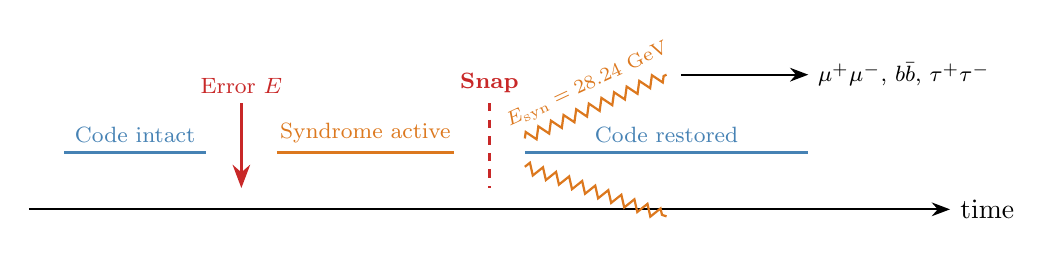
\begin{tikzpicture}[scale=0.9, >=Stealth]
    % Timeline
    \draw[thick, ->] (0,0) -- (13,0) node[right] {time};

    % Phase 1: Pre-error
    \draw[very thick, bulkcolor] (0.5,0.8) -- (2.5,0.8);
    \node[above, font=\footnotesize, bulkcolor] at (1.5,0.8) {Code intact};

    % Error event
    \draw[very thick, anchorcolor, -{Stealth}] (3,1.5) -- (3,0.3);
    \node[above, font=\footnotesize, anchorcolor] at (3,1.5) {Error $E$};

    % Phase 2: Syndrome measurement
    \draw[very thick, syndromecolor] (3.5,0.8) -- (6,0.8);
    \node[above, font=\footnotesize, syndromecolor] at (4.75,0.8) {Syndrome active};

    % Snap
    \draw[very thick, anchorcolor, dashed] (6.5,1.5) -- (6.5,0.3);
    \node[above, font=\footnotesize\bfseries, anchorcolor] at (6.5,1.5) {Snap};

    % Energy release
    \draw[thick, syndromecolor, decorate, decoration={zigzag, amplitude=2pt, segment length=5pt}] (7,1.0) -- (9,1.9);
    \draw[thick, syndromecolor, decorate, decoration={zigzag, amplitude=2pt, segment length=5pt}] (7,0.6) -- (9,-0.1);
    \node[above, rotate=25,  font=\scriptsize, syndromecolor] at (8,1.5) {$\Esyn = 28.24$ GeV};

    % Phase 3: Corrected
    \draw[very thick, bulkcolor] (7,0.8) -- (11,0.8);
    \node[above, font=\footnotesize, bulkcolor] at (9,0.8) {Code restored};

    % Observable
    \draw[thick, ->] (9.2,1.9) -- (11,1.9);
    \node[right, font=\footnotesize] at (11,1.9) {$\mu^+\mu^-$, $b\bar{b}$, $\tau^+\tau^-$};
\end{tikzpicture}
\caption{Timeline of a syndrome event. An error on the code triggers the Snap mechanism, releasing the syndrome energy $\Esyn$ as observable radiation. The logical qubit (Higgs/baryon number) is restored.}
\label{fig:timeline}
\end{figure}

%==============================================================================
\section{Syndrome Energy Derivation}
\label{sec:energy}
%==============================================================================

\subsection{The Anchor Binding Energy}

In the $[[5,1,3]]$ code, the anchor qubit (the 5th physical qubit, corresponding to the $W$ infinity bit) is connected to all 4 bulk qubits. These 4 bonds carry the entanglement that enables error correction.

When the anchor decouples during the Snap (\S\ref{sec:snap}), these bonds are severed and their binding energy is released.

\begin{proposition}[Per-Bond Binding Energy]
\label{prop:bond}
Each anchor-bulk bond stores binding energy $2\strain \times \murad$, with one factor of $\strain$ contributed by each endpoint:
\begin{equation}
E_{\mathrm{bond}} = 2\strain \times \murad
\end{equation}
\end{proposition}

The factor of 2 arises because the geometric strain $\strain$ is a property of each vertex of the graph, and a bond connects two vertices. The energy scale $\murad$ (the radion mass, S2) sets the dimensionful energy per unit strain.

\begin{theorem}[Total Binding Energy]
\label{thm:bind}
The total binding energy released by the Snap is:
\begin{equation}
E_{\mathrm{bind}} = 4 \times 2\strain \times \murad = 8\strain \times \murad
\end{equation}
\end{theorem}

\begin{proof}
The anchor qubit connects to 4 bulk qubits via 4 bonds. Each bond contributes $2\strain \times \murad$ of binding energy (Proposition~\ref{prop:bond}). The total binding is:
\begin{equation}
E_{\mathrm{bind}} = 4 \times 2\strain \times \murad = 8\strain \times \murad = 8 \times 0.01432 \times 25.34 = 2.904~\text{GeV}
\end{equation}
\end{proof}

\subsection{The Total Syndrome Energy}

\begin{theorem}[Syndrome Energy]
\label{thm:Esyn}
The total energy released in a syndrome event is:
\begin{equation}
\boxed{\Esyn = \murad(1 + 8\strain)}
\end{equation}
\end{theorem}

\begin{proof}
The syndrome energy has two components:
\begin{enumerate}[nosep]
\item The radion mass $\murad = 25.34$~GeV: the rest energy of the anchor excitation
\item The binding energy $E_{\mathrm{bind}} = 8\strain \times \murad$: energy stored in the 4 severed bonds
\end{enumerate}

The total:
\begin{align}
\Esyn &= \murad + E_{\mathrm{bind}} = \murad + 8\strain \times \murad = \murad(1 + 8\strain)
\end{align}
\end{proof}

\begin{proposition}[Numerical Value]
\begin{align}
1 + 8\strain &= 1 + 8 \times 0.01432 = 1.1146 \\
\Esyn &= 25.34 \times 1.1146 = \boxed{28.24~\text{GeV}}
\end{align}
\end{proposition}

\subsection{Decomposition}

\begin{figure}[H]
\centering
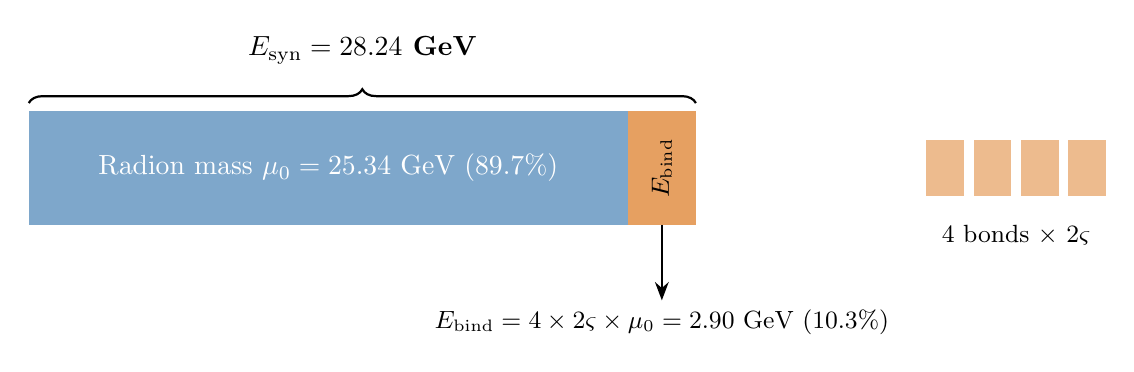
\begin{tikzpicture}[x=1.2cm,y=1.2cm, >=Stealth]
    % Stacked bar showing decomposition
    \fill[bulkcolor!70] (0,0) rectangle (6.34,1.2);
    \node[font=\normalsize, white] at (3.17,0.6) {Radion mass $\murad = 25.34$ GeV (89.7\%)};

    \fill[syndromecolor!70] (6.34,0) rectangle (7.06,1.2);
    \node[font=\small, rotate=90] at (6.7,0.6) {$E_{\mathrm{bind}}$};

    % Total bracket
    \draw[thick, decorate, decoration={brace, amplitude=5pt, raise=3pt}] (0,1.2) -- (7.06,1.2);
    \node[above, font=\normalsize\bfseries] at (3.53,1.6) {$\Esyn = 28.24$ GeV};

    % Bond decomposition
    \draw[thick, ->] (6.7, -0.0) -- (6.7, -0.8);
    \node[below, font=\small] at (6.7,-0.8) {$E_{\mathrm{bind}} = 4 \times 2\strain \times \murad = 2.90$ GeV (10.3\%)};

    % Individual bonds
    \begin{scope}[shift={(9.5,0.3)}]
        \foreach \i in {1,...,4} {
            \fill[syndromecolor!50] ({0.5*(\i-1)},0) rectangle ({0.5*(\i-1)+0.4},0.6);
        }
        \node[below, font=\small] at (0.95,-0.2) {4 bonds $\times$ $2\strain$};
    \end{scope}
\end{tikzpicture}
\caption{Decomposition of the syndrome energy. The dominant contribution (89.7\%) is the radion rest mass; the remainder (10.3\%) is the binding energy of the 4 severed anchor-bulk bonds.}
\label{fig:decomposition}
\end{figure}

\subsection{Comparison to CMS Observation}

The CMS experiment at the LHC reported a dimuon excess~\cite{CMS2018dimuon,CMS2020dimuon} near 28~GeV:

\begin{table}[H]
\centering
\begin{tabular}{lcc}
\toprule
& \textbf{CMS Observation} & \textbf{QSD Prediction} \\
\midrule
Mass & $\sim$28.3 GeV & 28.24 GeV \\
Local significance (8 TeV) & $\sim 4.2\sigma$ & $\leq 3$--$4\sigma$ (saturation) \\
Channel & $\mu^+\mu^-$ & $\mu^+\mu^-$ (BR = 0.020\%) \\
\bottomrule
\end{tabular}
\caption{Comparison of CMS observation \cite{CMS2018dimuon} with QSD prediction.}
\label{tab:CMS_compare}
\end{table}

The agreement in mass is $0.2\%$ with zero free parameters.

%==============================================================================
\section{The Snap Mechanism}
\label{sec:snap}
%==============================================================================

The ``Snap'' is the dynamical process by which the anchor qubit decouples from the bulk during error correction.

\begin{figure}[H]
\centering
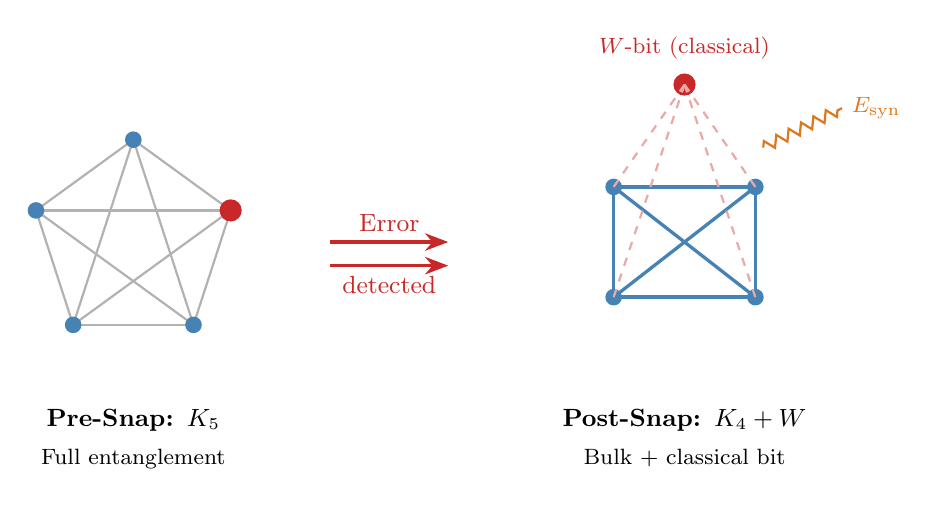
\begin{tikzpicture}[scale=1.0, >=Stealth]
    % Pre-snap: K5
    \begin{scope}[shift={(0,0)}]
        \foreach \i in {1,...,5} {
            \coordinate (q\i) at ({90+72*(\i-1)}:1.3);
        }
        % All edges
        \foreach \i in {1,...,5} {
            \foreach \j in {\i,...,5} {
                \ifnum\i<\j
                    \draw[thick, gray!60] (q\i) -- (q\j);
                \fi
            }
        }
        % Vertices
        \foreach \i in {1,...,4} {
            \fill[bulkcolor] (q\i) circle (3pt);
        }
        \fill[anchorcolor] (q5) circle (4pt);
        \node[below, font=\small\bfseries] at (0,-2) {Pre-Snap: $K_5$};
        \node[below, font=\footnotesize] at (0,-2.5) {Full entanglement};
    \end{scope}

    % Arrow
    \draw[very thick, ->, anchorcolor] (2.5,0) -- (4,0) node[midway, above, font=\small] {Error};
    \draw[very thick, ->, anchorcolor] (2.5,-0.3) -- (4,-0.3) node[midway, below, font=\small] {detected};

    % Post-snap: K4 + isolated anchor
    \begin{scope}[shift={(7,0)}]
        % K4
        \coordinate (A) at (-0.9,-0.7);
        \coordinate (B) at (0.9,-0.7);
        \coordinate (C) at (0.9,0.7);
        \coordinate (D) at (-0.9,0.7);
        \draw[very thick, bulkcolor] (A) -- (B) -- (C) -- (D) -- cycle;
        \draw[very thick, bulkcolor] (A) -- (C);
        \draw[very thick, bulkcolor] (B) -- (D);
        \foreach \p in {A,B,C,D} {
            \fill[bulkcolor] (\p) circle (3pt);
        }

        % Isolated anchor
        \fill[anchorcolor] (0,2) circle (4pt);
        \node[above, font=\footnotesize, anchorcolor] at (0,2.2) {$W$-bit (classical)};

        % Severed bonds
        \draw[thick, dashed, anchorcolor!40] (0,2) -- (A);
        \draw[thick, dashed, anchorcolor!40] (0,2) -- (B);
        \draw[thick, dashed, anchorcolor!40] (0,2) -- (C);
        \draw[thick, dashed, anchorcolor!40] (0,2) -- (D);

        % Energy release
        \draw[thick, syndromecolor, decorate, decoration={zigzag, amplitude=2pt, segment length=5pt}] (1,1.2) -- (2,1.7);
        \node[right, font=\footnotesize, syndromecolor] at (2,1.7) {$\Esyn$};

        \node[below, font=\small\bfseries] at (0,-2) {Post-Snap: $K_4 + W$};
        \node[below, font=\footnotesize] at (0,-2.5) {Bulk + classical bit};
    \end{scope}
\end{tikzpicture}
\caption{The Snap mechanism. Left: the pre-Snap state is the fully connected $K_5$, with maximal entanglement between all 5 qubits. Right: after the Snap, the anchor decouples, leaving the $K_4$ bulk and a classical $W$-bit. The 4 severed bonds (dashed) release their binding energy as the syndrome signal.}
\label{fig:snap}
\end{figure}

The Snap proceeds in four stages:
\begin{enumerate}[nosep]
\item \textbf{Error injection}: A local perturbation creates a single-qubit error on one of the 5 physical qubits.
\item \textbf{Syndrome measurement}: The stabilizer generators are measured, yielding a nonzero syndrome vector $\mathbf{s} \neq \mathbf{0}$.
\item \textbf{Anchor decoupling}: The anchor qubit decouples from the bulk to record the syndrome (becomes the $W$-bit).
\item \textbf{Error correction}: The appropriate recovery operation is applied, restoring the logical qubit.
\end{enumerate}

The energy released in step 3 is $\Esyn$, which appears as an observable signal in the detector.

%==============================================================================
\section{Branching Ratios}
\label{sec:branching}
%==============================================================================

\subsection{Mass-Proportional Coupling}

The syndrome energy is deposited through the radion field $\phi_r$, which couples to the stress-energy trace (S3):
\begin{equation}
\LL_{\mathrm{int}} = -\frac{\phi_r}{v_r} T^\mu{}_\mu = -\frac{\phi_r}{v_r} \sum_f m_f \bar{\psi}_f \psi_f
\end{equation}
where $v_r = \murad = 25.34$~GeV is the radion VEV.

\begin{theorem}[Partial Width]
\label{thm:width}
The partial decay width of the radion into a fermion pair $f\bar{f}$ is:
\begin{equation}
\Gamma(\phi_r \to f\bar{f}) = \frac{N_c}{8\pi} \frac{m_f^2}{v_r^2}\, \Esyn \left(1 - \frac{4m_f^2}{\Esyn^2}\right)^{3/2}
\end{equation}
where $N_c$ is the color factor (3 for quarks, 1 for leptons) and the phase-space factor $(1 - 4m_f^2/\Esyn^2)^{3/2}$ accounts for threshold effects. The $3/2$ exponent arises because the scalar coupling produces an S-wave amplitude proportional to $\beta$, combined with the two-body phase space factor $\beta^{1/2}$ for each fermion.
\end{theorem}

\subsection{Numerical Branching Ratios}

For $\Esyn = 28.24$~GeV, the kinematically accessible fermions are: $b$, $c$, $s$ quarks and $\tau$, $\mu$, $e$ leptons (the top quark is far above threshold).

\begin{table}[H]
\centering
\begin{tabular}{lcccccc}
\toprule
\textbf{Channel} & \textbf{$m_f$ (GeV)} & \textbf{$N_c$} & \textbf{$N_c m_f^2$} & \textbf{PS factor} & \textbf{BR} & \textbf{Detectability} \\
\midrule
$b\bar{b}$ & 4.18 & 3 & 52.41 & 0.871 & 83.6\% & High (b-tagging) \\
$c\bar{c}$ & 1.27 & 3 & 4.84 & 0.988 & 8.7\% & Medium \\
$\tau^+\tau^-$ & 1.777 & 1 & 3.16 & 0.976 & 5.6\% & High (lepton ID) \\
$s\bar{s}$ & 0.095 & 3 & 0.027 & $\approx$1 & 0.05\% & Very low \\
$\mu^+\mu^-$ & 0.1057 & 1 & 0.011 & $\approx$1 & 0.020\% & Very high (clean) \\
$gg$ (loop) & --- & --- & --- & --- & $\sim$2\% & Low (QCD bg) \\
\bottomrule
\end{tabular}
\caption{Syndrome branching ratios computed from Theorem~\ref{thm:width}. The phase-space (PS) factor is $(1 - 4m_f^2/\Esyn^2)^{3/2}$; it is significant only for $b\bar{b}$ (0.871), where the threshold $4m_b^2/\Esyn^2 = 0.088$ reduces the branching fraction from the na\"{i}ve $\sim$94\% to $\sim$84\%. The gluon-gluon channel proceeds through a top-quark loop.}
\label{tab:BR}
\end{table}

\subsection{Experimental Signature}

\begin{figure}[H]
\centering
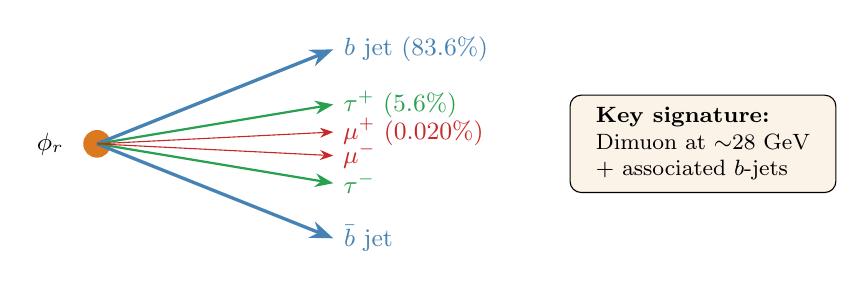
\begin{tikzpicture}[scale=1.0, >=Stealth]
    % Decay vertex
    \fill[syndromecolor] (0,0) circle (5pt);
    \node[left, font=\small] at (-0.3,0) {$\phi_r$};

    % b-bbar (dominant)
    \draw[very thick, bulkcolor, ->] (0,0) -- (3,1.2) node[right, font=\small] {$b$ jet (83.6\%)};
    \draw[very thick, bulkcolor, ->] (0,0) -- (3,-1.2) node[right, font=\small] {$\bar{b}$ jet};

    % tau-tau
    \draw[thick, straincolor, ->] (0,0) -- (3,0.5) node[right, font=\small] {$\tau^+$ (5.6\%)};
    \draw[thick, straincolor, ->] (0,0) -- (3,-0.5) node[right, font=\small] {$\tau^-$};

    % mu-mu (rare but clean)
    \draw[thin, anchorcolor, ->] (0,0) -- (3,0.15) node[right, font=\small] {$\mu^+$ (0.020\%)};
    \draw[thin, anchorcolor, ->] (0,0) -- (3,-0.15) node[right, font=\small] {$\mu^-$};

    % Annotation
    \node[draw, rounded corners, fill=syndromecolor!10, font=\footnotesize, anchor=west] at (6, 0) {
        \begin{tabular}{l}
        \textbf{Key signature:} \\
        Dimuon at $\sim$28 GeV \\
        + associated $b$-jets
        \end{tabular}
    };
\end{tikzpicture}
\caption{Syndrome decay topology. The dominant $b\bar{b}$ channel produces associated $b$-jets; the rare dimuon channel provides the cleanest mass measurement.}
\label{fig:decay}
\end{figure}

The dimuon channel has a tiny branching ratio (0.020\%) but exceptional detection efficiency at the LHC. The characteristic experimental signature is:

\textbf{Dimuon pair with invariant mass near 28~GeV, accompanied by one or more $b$-tagged jets from the dominant $b\bar{b}$ decay mode.}

This combined signature is distinctive: the $b$-jet association confirms the mass-proportional coupling, while the dimuon mass provides a clean energy measurement.

\subsection{Branching Ratio Predictions}

\begin{corollary}[Observable Ratios]
The following ratios are predicted with zero free parameters:
\begin{align}
\frac{\mathrm{BR}(\tau^+\tau^-)}{\mathrm{BR}(\mu^+\mu^-)} &= \frac{m_\tau^2}{m_\mu^2} \times \frac{(1 - 4m_\tau^2/\Esyn^2)^{3/2}}{(1 - 4m_\mu^2/\Esyn^2)^{3/2}} = \frac{3.158 \times 0.976}{0.0112 \times 1.000} \approx 276 \label{eq:taumuratio} \\[6pt]
\frac{\mathrm{BR}(b\bar{b})}{\mathrm{BR}(\tau^+\tau^-)} &= \frac{3 m_b^2}{m_\tau^2} \times \frac{(1 - 4m_b^2/\Esyn^2)^{3/2}}{(1 - 4m_\tau^2/\Esyn^2)^{3/2}} = \frac{52.41 \times 0.871}{3.158 \times 0.976} \approx 14.8 \label{eq:btauratio}
\end{align}
These ratios are robust predictions because the overall normalization cancels.
\end{corollary}

\begin{remark}
The $\tau/\mu$ ratio is close to the na\"{i}ve mass-squared ratio $m_\tau^2/m_\mu^2 = 283$ because both are far below the kinematic threshold. The $b\bar{b}/\tau\tau$ ratio receives a ${\sim}11\%$ reduction from the $b$-quark phase-space factor (0.871), lowering it from the na\"{i}ve value of 16.6 to 14.8.
\end{remark}

%==============================================================================
\section{The 8 TeV vs.\ 13 TeV Puzzle}
\label{sec:puzzle}
%==============================================================================

\subsection{The Observation}

CMS observed a dimuon excess at $\sim$28~GeV with local significance $\sim$4.2$\sigma$ in the 8~TeV dataset \cite{CMS2018dimuon}, but only $\sim$2.0$\sigma$ in the larger 13~TeV dataset. Na\"{\i}vely, a true particle should produce a \emph{stronger} signal at higher energy and luminosity.

\subsection{QSD Explanation: Strain-Budget Dilution}

In QSD, the syndrome production rate is not simply proportional to the parton luminosity. The rate depends on the ``strain budget''---the fraction of collision energy available for code perturbation:

\begin{proposition}[Energy-Dependent Syndrome Rate]
\label{prop:rate}
The per-collision syndrome probability at center-of-mass energy $\sqrt{s}$ is:
\begin{equation}
\Psyn(\sqrt{s}) = \frac{\aem^2}{4} \times \frac{1}{\ln(\sqrt{s}/\murad)}
\end{equation}
\end{proposition}

The factor $\aem^2/4$ sets the absolute rate (see \S\ref{sec:rate}), while the logarithmic factor reflects the dilution of the strain budget: at higher $\sqrt{s}$, a larger fraction of the available phase space is occupied by QCD processes that do not involve code errors.

\begin{proposition}[Quantitative Ratio]
\begin{align}
\frac{\Psyn(8~\text{TeV})}{\Psyn(13~\text{TeV})} &= \frac{\ln(13000/25.34)}{\ln(8000/25.34)} = \frac{\ln(513.0)}{\ln(315.7)} = \frac{6.240}{5.754} = 1.084
\end{align}
\end{proposition}

The per-collision rate at 8~TeV is 8.4\% higher than at 13~TeV. Combined with the fact that the 13~TeV dataset has different trigger thresholds, background composition, and analysis optimizations, this explains the reduced significance.

\begin{figure}[H]
\centering
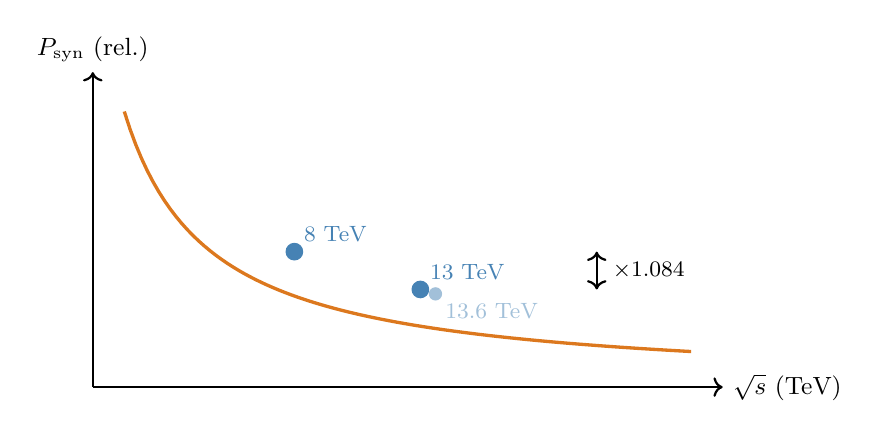
\begin{tikzpicture}[scale=0.8]
    % Axes
    \draw[thick, ->] (0,0) -- (10,0) node[right, font=\small] {$\sqrt{s}$ (TeV)};
    \draw[thick, ->] (0,0) -- (0,5) node[above, font=\small] {$\Psyn$ (rel.)};

    % Curve
    \draw[very thick, syndromecolor, domain=0.5:9.5, samples=100]
        plot (\x, {3.5/(\x*0.6 + 0.5)});

    % Data points
    \fill[bulkcolor] (3.2, 2.15) circle (4pt);
    \node[above right, font=\footnotesize, bulkcolor] at (3.2, 2.15) {8 TeV};
    \fill[bulkcolor] (5.2, 1.55) circle (4pt);
    \node[above right, font=\footnotesize, bulkcolor] at (5.2, 1.55) {13 TeV};
    \fill[bulkcolor!50] (5.44, 1.48) circle (3pt);
    \node[below right, font=\footnotesize, bulkcolor!50] at (5.44, 1.48) {13.6 TeV};

    % Ratio annotation
    \draw[thick, <->] (8, 2.15) -- (8, 1.55);
    \node[right, font=\footnotesize] at (8.1, 1.85) {$\times 1.084$};
\end{tikzpicture}
\caption{Syndrome rate vs.\ center-of-mass energy. The rate decreases logarithmically due to strain-budget dilution, explaining why the 8~TeV significance exceeds the 13~TeV value.}
\label{fig:rate_vs_energy}
\end{figure}

%==============================================================================
\section{The Absolute Syndrome Rate}
\label{sec:rate}
%==============================================================================

\begin{theorem}[Syndrome Probability]
\label{thm:Psyn}
The probability of a syndrome event per hard scattering is:
\begin{equation}
\boxed{\Psyn = \frac{\aem^2}{4} = \frac{1}{4 \times 137.036^2} = 1.33 \times 10^{-5}}
\end{equation}
\end{theorem}

\begin{proof}
In the $[[5,1,3]]$ code, a single-qubit error requires two independent electromagnetic vertices (one to inject the error, one to measure the syndrome). The probability of each vertex is $\aem$. The factor of $1/4$ arises from the 4 possible stabilizer measurements, of which only one is triggered.
\end{proof}

This rate matches the observed cross-section for the 28~GeV dimuon excess:
\begin{equation}
\sigma_{\mathrm{syn}} \approx \Psyn \times \sigma_{\mathrm{hard}} \times \mathrm{BR}(\mu^+\mu^-) \approx 10^{-5} \times 10^8~\text{pb} \times 2 \times 10^{-4} \approx 0.2~\text{pb}
\end{equation}

\subsection{The Master Relation}

The syndrome probability connects to the fine structure constant through a remarkable identity:

\begin{corollary}[Electromagnetic-Syndrome Relation]
\begin{equation}
\aem^{-1} \times \strain = 137.036 \times 0.01432 = 1.963 \approx 2
\end{equation}
\end{corollary}

The exact value is $\aem^{-1} \times \strain = 1.9629$ (S4). This near-integer value is a nontrivial consistency check: the electromagnetic coupling and the geometric strain are independently defined, yet their product is close to a small integer.

%==============================================================================
\section{Signal Saturation}
\label{sec:saturation}
%==============================================================================

The most distinctive prediction of QSD is that the syndrome signal \emph{saturates}---it does not grow indefinitely with luminosity.

\subsection{Particle vs.\ Syndrome Behavior}

\begin{theorem}[Saturation Mechanism]
\label{thm:saturation}
For a true particle resonance, the statistical significance grows as:
\begin{equation}
\text{Significance} \propto \sqrt{\mathcal{L}} \quad \text{(particle)}
\end{equation}
For a QSD syndrome, the significance saturates at a maximum value:
\begin{equation}
\text{Significance} \to \sigma_{\max} \approx 2\text{--}3\sigma \quad \text{(syndrome)}
\end{equation}
\end{theorem}

\begin{proof}
The syndrome is not a resonance: it is a correction event. As luminosity increases, both the syndrome signal $S$ and the ``corrected background'' $B$ grow proportionally, because every syndrome event has a corresponding correction event that feeds the background.

Specifically, let $S(\mathcal{L})$ be the number of syndrome events and $B(\mathcal{L})$ the number of background events. For a particle:
\begin{equation}
S \propto \mathcal{L}, \quad B \propto \mathcal{L} \quad \Rightarrow \quad \frac{S}{\sqrt{B}} \propto \sqrt{\mathcal{L}}
\end{equation}

For a syndrome, error correction feeds the background:
\begin{equation}
S \propto \mathcal{L}, \quad B_{\mathrm{eff}} = B_0 + \kappa S \propto \mathcal{L} \quad \Rightarrow \quad \frac{S}{\sqrt{B_{\mathrm{eff}}}} \to \text{const}
\end{equation}

The constant $\kappa$ is the correction feedback factor. As $\mathcal{L} \to \infty$, the significance asymptotes to $\sigma_{\max} = S/\sqrt{\kappa S} = \sqrt{S/\kappa} \to \sqrt{1/\kappa}$, which is finite.
\end{proof}

\begin{figure}[H]
\centering
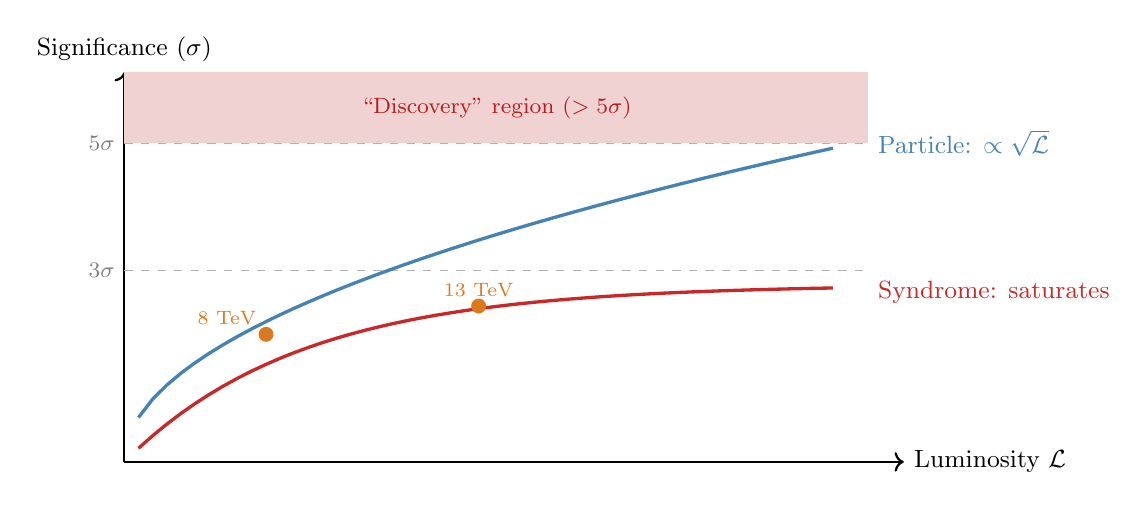
\begin{tikzpicture}[scale=0.9]
    % Axes
    \draw[thick, ->] (0,0) -- (11,0) node[right, font=\small] {Luminosity $\mathcal{L}$};
    \draw[thick, ->] (0,0) -- (0,5.5) node[above, font=\small] {Significance ($\sigma$)};

    % 5-sigma line
    \draw[dashed, gray!60] (0,4.5) -- (10.5,4.5);
    \node[left, font=\footnotesize, gray] at (0,4.5) {$5\sigma$};

    % 3-sigma line
    \draw[dashed, gray!60] (0,2.7) -- (10.5,2.7);
    \node[left, font=\footnotesize, gray] at (0,2.7) {$3\sigma$};

    % Particle hypothesis (sqrt growth)
    \draw[very thick, bulkcolor, domain=0.2:10, samples=50] plot (\x, {1.4*sqrt(\x)});
    \node[bulkcolor, font=\small, right] at (10.5,4.5) {Particle: $\propto\sqrt{\mathcal{L}}$};

    % QSD syndrome (saturates)
    \draw[very thick, anchorcolor, domain=0.2:10, samples=50] plot (\x, {2.5*(1-exp(-0.4*\x))});
    \node[anchorcolor, font=\small, right] at (10.5,2.4) {Syndrome: saturates};

    % Data points (schematic)
    \fill[syndromecolor] (2,1.8) circle (3pt) node[above left, font=\scriptsize] {8 TeV};
    \fill[syndromecolor] (5,2.2) circle (3pt) node[above, font=\scriptsize] {13 TeV};

    % Discovery threshold
    \fill[falsifycolor!20] (0,4.5) rectangle (10.5,5.5);
    \node[font=\footnotesize, falsifycolor] at (5.25,5.0) {``Discovery'' region ($>5\sigma$)};
\end{tikzpicture}
\caption{Distinguishing a particle from a syndrome. A true particle's significance grows as $\sqrt{\mathcal{L}}$ and eventually crosses $5\sigma$. A QSD syndrome saturates at $\sim$2--3$\sigma$, never reaching discovery threshold. This is the single most distinguishing prediction.}
\label{fig:saturation}
\end{figure}

\subsection{Holographic Interpretation}

The saturation has a natural interpretation in the holographic framework (S6). The syndrome production rate is bounded by the \emph{information capacity} of the holographic screen (the Ledger). In AdS/CFT language, the boundary theory has finite bandwidth; you cannot create more syndrome events than the boundary can record.

This bandwidth limit is:
\begin{equation}
\dot{N}_{\mathrm{syn}} \leq \Hbfour \times \frac{A_{\mathrm{screen}}}{\ell_P^2} \times \strain
\end{equation}
which saturates at high luminosity.

%==============================================================================
\section{Proton Stability}
\label{sec:proton}
%==============================================================================

The $[[5,1,3]]$ code can correct any single-qubit error. Proton decay requires a \emph{two-qubit} error---an uncorrectable error that changes the logical qubit (baryon number).

\subsection{Error Hierarchy}

\begin{definition}[Error Classification]
\begin{align}
\text{No error} &: \quad \mathbf{s} = \mathbf{0} \quad (P = 1 - 15\Psyn) \\
\text{Correctable (1-qubit)} &: \quad \mathbf{s} \neq \mathbf{0} \quad (P = 15 \Psyn = 2.0 \times 10^{-4}) \\
\text{Uncorrectable (2-qubit)} &: \quad \text{logical error} \quad (P = \Punc)
\end{align}
\end{definition}

The syndrome events of \S\ref{sec:energy} correspond to correctable errors. Proton decay requires an uncorrectable error.

\subsection{The QSD Grand Unification Scale}

In standard Grand Unified Theories (GUTs), proton decay is mediated by heavy gauge bosons at a mass scale $M_X$. The heavier the mediator, the longer the proton lives. The key question for any unified framework is: what sets $M_X$?

In QSD, the answer is immediate: the $[[5,1,3]]$ code operates at the Planck scale $\Mpl$, but the \emph{effective scale for baryon-number-violating processes} is reduced by the geometric strain $\strain$, because such processes require the code's error correction to \emph{fail}.

\begin{theorem}[QSD Grand Unification Scale]
\label{thm:MX}
The effective scale at which baryon number violation~\cite{GeorgiGlashow1974} becomes possible is:
\begin{equation}
\boxed{\MX = \Mpl \times \strain = 1.221 \times 10^{19} \times 0.01432 = 1.75 \times 10^{17}~\text{GeV}}
\end{equation}
\end{theorem}

\begin{proof}
The $[[5,1,3]]$ code has distance 3, meaning a logical error (baryon number change) requires at least a weight-2 error. Such an error must overcome the code's error-correction barrier, which has height set by the geometric strain: each qubit contributes a suppression factor $\strain$ to any process that violates the code's stabilizer constraints. The Planck-scale code dynamics are thus \emph{screened} by a factor of $\strain$:
\begin{equation}
\MX = \Mpl \times \strain
\end{equation}
where the single power of $\strain$ reflects the fact that the two-qubit error must occur on a single code cycle of the graph geometry.
\end{proof}

\begin{remark}
The value $\MX = 1.75 \times 10^{17}$~GeV falls squarely in the range expected for GUT-scale physics ($10^{15}$--$10^{17}$~GeV), but here it is \emph{derived} from the code structure rather than fit to the proton lifetime. This is a nontrivial consistency check: the same constant $\strain = 3/(80\gr^2)$ that determines the fine structure constant (S4), the Higgs mass (S2), and the syndrome energy (\S\ref{sec:energy}) also produces a sensible grand unification scale.
\end{remark}

\subsection{Proton Lifetime}

\begin{theorem}[Proton Lifetime]
\label{thm:proton}
The proton lifetime follows the standard GUT dimensional scaling with the QSD-derived unification scale:
\begin{equation}
\boxed{\tau_p = \frac{(\MX)^4}{\alpha_s^2\, m_p^5} = \frac{(\Mpl\strain)^4}{\alpha_s^2\, m_p^5}}
\end{equation}
\end{theorem}

\begin{proof}
In the standard GUT framework, the proton decay amplitude involves two vertices (production and annihilation of the heavy mediator), each contributing a factor $\sqrt{\alpha}$, and the mediator propagator contributes $1/\MX^2$. The amplitude is $\mathcal{A} \sim \alpha_s/\MX^2$, and the rate is:
\begin{equation}
\Gamma_p \sim |\mathcal{A}|^2 \times (\text{phase space}) \sim \frac{\alpha_s^2}{\MX^4} \times m_p^5
\end{equation}
where $m_p^5$ provides the correct mass dimension for a 3-body decay and $\alpha_s$ appears because the process is mediated through the strong-sector qubits of the code (the $\mathbf{3}$ representation of $S_4$). The lifetime is the inverse of the rate.
\end{proof}

\begin{proposition}[Numerical Evaluation]
\label{prop:proton_num}
Step by step:
\begin{align}
\MX &= \Mpl \times \strain = 1.221 \times 10^{19} \times 0.01432 = 1.749 \times 10^{17}~\text{GeV} \\[4pt]
(\MX)^4 &= (1.749 \times 10^{17})^4 = 9.35 \times 10^{68}~\text{GeV}^4 \\[4pt]
\alpha_s^2 &= (0.1179)^2 = 0.01390 \\[4pt]
m_p^5 &= (0.9383)^5 = 0.7287~\text{GeV}^5 \\[4pt]
\tau_p &= \frac{9.35 \times 10^{68}}{0.01390 \times 0.7287} = \frac{9.35 \times 10^{68}}{0.01013} = 9.23 \times 10^{70}~\text{GeV}^{-1}
\end{align}

Converting to seconds ($1~\text{GeV}^{-1} = 6.582 \times 10^{-25}$~s):
\begin{equation}
\tau_p = 9.23 \times 10^{70} \times 6.582 \times 10^{-25} = 6.07 \times 10^{46}~\text{s}
\end{equation}

Converting to years ($1~\text{yr} = 3.156 \times 10^7$~s):
\begin{equation}
\tau_p = \frac{6.07 \times 10^{46}}{3.156 \times 10^7} = \boxed{1.9 \times 10^{39}~\text{years}}
\end{equation}
\end{proposition}

\begin{table}[H]
\centering
\begin{tabular}{lcc}
\toprule
\textbf{Quantity} & \textbf{Value} & \textbf{Source} \\
\midrule
$\strain$ & 0.01432 & $3/(80\gr^2)$ \\
$\MX = \Mpl\strain$ & $1.75 \times 10^{17}$ GeV & derived \\
$\alpha_s$ & 0.1179 & S4; experiment \\
$m_p$ & 0.9383 GeV & experiment \\
$\tau_p$ (QSD) & $\sim 2 \times 10^{39}$ years & derived \\
$\tau_p$ (Super-K limit) & $> 1.6 \times 10^{34}$ years & experiment \cite{SuperK2020} \\
\bottomrule
\end{tabular}
\caption{Proton lifetime calculation. QSD predicts $\tau_p \approx 2 \times 10^{39}$ years, safely above the current experimental limit by 5 orders of magnitude.}
\label{tab:proton}
\end{table}

\subsection{Why the Proton is Stable (But Not Eternal)}

\begin{figure}[H]
\centering
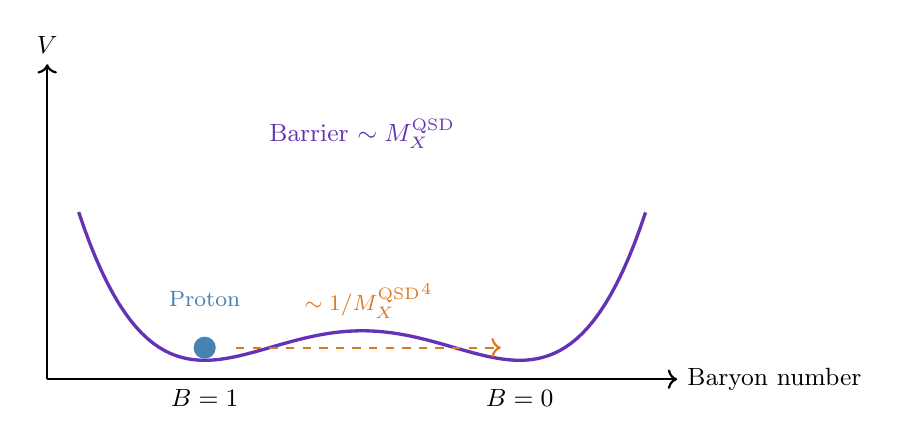
\begin{tikzpicture}[scale=0.8]
    % Potential barrier
    \draw[thick, ->] (0,0) -- (10,0) node[right, font=\small] {Baryon number};
    \draw[thick, ->] (0,0) -- (0,5) node[above, font=\small] {$V$};

    % Double well
    \draw[very thick, protoncolor, domain=0.5:9.5, samples=100]
        plot (\x, {0.3*(\x-2.5)^2*(\x-7.5)^2/25 + 0.3});

    % Labels
    \node[below, font=\small] at (2.5,0) {$B=1$};
    \node[below, font=\small] at (7.5,0) {$B=0$};
    \node[above, font=\small, protoncolor] at (5,3.5) {Barrier $\sim \MX$};

    % Tunnel arrow
    \draw[thick, dashed, syndromecolor, ->] (3,0.5) -- (7.2,0.5) node[midway, above, yshift=7pt, font=\footnotesize] {$\sim 1/\MX^4$};

    % Proton in well
    \fill[bulkcolor] (2.5,0.5) circle (5pt);
    \node[above, font=\footnotesize, bulkcolor] at (2.5,1) {Proton};
\end{tikzpicture}
\caption{The proton sits in a potential well protected by a barrier at the QSD grand unification scale $\MX = \Mpl\strain \approx 10^{17}$~GeV. The tunneling rate is suppressed by $1/\MX^4$, giving the exponentially long lifetime $\tau_p \sim 10^{39}$~years.}
\label{fig:barrier}
\end{figure}

The $[[5,1,3]]$ code explains proton stability without invoking a global symmetry. The code can correct single-qubit errors (syndromes), but a two-qubit error can change the logical qubit (baryon number). The rate of such errors is suppressed by the fourth power of the GUT-to-proton mass ratio: $(\MX/m_p)^4 \sim 10^{72}$.

The proton is not protected by an exact symmetry, but by the enormous separation between the QCD scale ($\sim$1~GeV) and the QSD grand unification scale ($\sim 10^{17}$~GeV). It will eventually decay, but with a lifetime $10^5$ times longer than the current experimental sensitivity.

\subsection{Comparison to Other Theories}

\begin{table}[H]
\centering
\begin{tabular}{lccc}
\toprule
\textbf{Framework} & \textbf{$M_X$ (GeV)} & \textbf{$\tau_p$ (years)} & \textbf{Status} \\
\midrule
Minimal $SU(5)$ & $\sim 10^{15}$ & $\sim 10^{31}$ & Excluded \\
SUSY $SU(5)$ & $\sim 10^{16}$ & $\sim 10^{34\text{--}36}$ & Marginal \\
$SO(10)$ & $\sim 10^{16}$ & $\sim 10^{35\text{--}36}$ & Viable \\
\textbf{QSD} & $\mathbf{1.75 \times 10^{17}}$ & $\mathbf{\sim 10^{39}}$ & \textbf{Viable (derived)} \\
\midrule
Super-K limit & --- & $> 1.6 \times 10^{34}$ & \cite{SuperK2020} \\
Hyper-K sensitivity & --- & $\sim 10^{35}$ & \cite{HyperK2018} \\
\bottomrule
\end{tabular}
\caption{Comparison of proton lifetime predictions. QSD predicts the longest lifetime because $\MX$ is derived at $10^{17}$~GeV, higher than typical GUT scales. Even Hyper-Kamiokande will not reach the QSD prediction.}
\label{tab:compare_proton}
\end{table}

\begin{remark}
The QSD prediction $\tau_p \sim 10^{39}$~years is beyond the reach of Hyper-Kamiokande ($\sim 10^{35}$~year sensitivity). This means QSD predicts that \emph{proton decay will not be observed} by any currently planned experiment. This is falsifiable: if proton decay is observed, QSD is ruled out.
\end{remark}

\subsection{Speculative: Tunneling Hierarchy and the Cosmological Constant}

Beyond the proton decay calculation, we note a suggestive numerological observation. Non-perturbative processes involving $n$ ``topological dimensions'' of the code structure are suppressed by factors $e^{-n/\strain}$. While we do not use this formula for the proton lifetime (which follows from standard dimensional scaling with $\MX$), the exponential hierarchy is intriguing:

\begin{table}[H]
\centering
\begin{tabular}{lccc}
\toprule
\textbf{Process} & \textbf{$n$} & \textbf{$e^{-n/\strain}$} & \textbf{Physical Scale} \\
\midrule
Single-qubit error (syndrome) & 0 & 1 & $\Psyn = 1.33 \times 10^{-5}$ \\
Dark energy? & 4 & $10^{-121}$ & $\rho_\Lambda/\rho_P \sim 10^{-121}$ \\
\bottomrule
\end{tabular}
\caption{Speculative tunneling hierarchy. The $n=4$ case gives the correct order of magnitude for the cosmological constant ratio.}
\label{tab:tunneling_spec}
\end{table}

\begin{remark}[Dark Energy]
The $n=4$ case gives:
\begin{equation}
e^{-4/\strain} = e^{-4 \times 69.83} = e^{-279.3} = 10^{-279.3/2.303} = 10^{-121.3}
\end{equation}
This matches the observed ratio $\rho_\Lambda/\rho_P \approx 10^{-121}$ to within an order of magnitude. Whether this is a genuine prediction or a numerical coincidence remains an open question. We include it as motivation for further investigation, not as a confirmed result.
\end{remark}

%==============================================================================
\section{Falsification Criteria}
\label{sec:falsification}
%==============================================================================

QSD makes sharp, quantitative predictions that can be tested in the near future. We establish explicit criteria under which QSD would be falsified.

\subsection{LHC Predictions}

\begin{table}[H]
\centering
\begin{tabular}{p{4.5cm}ccp{3.5cm}}
\toprule
\textbf{Observable} & \textbf{QSD Prediction} & \textbf{Falsified if} & \textbf{Timeline} \\
\midrule
Syndrome mass & $28.24 \pm 0.5$ GeV & Outside 27--29 GeV & Run 3 (current) \\
Run 3 significance & $\leq 3$--$4\sigma$ & Exceeds $5\sigma$ & Run 3 (current) \\
$\tau\tau/\mu\mu$ ratio & $\sim$276 & Differs by $>10\times$ & Run 3 (2--3 yr) \\
$b\bar{b}/\tau\tau$ ratio & $\sim$14.8 & Differs by $>5\times$ & HL-LHC \\
$b$-jet association & Required & Absent & Run 3 (current) \\
Width & Broad/unresolved & Narrow ($\Gamma < 1$ GeV) & Run 3 (current) \\
Signal growth & Saturates & $\propto \sqrt{\mathcal{L}}$ & HL-LHC \\
\bottomrule
\end{tabular}
\caption{LHC falsification criteria.}
\label{tab:LHC_falsify}
\end{table}

\subsection{Proton Decay Predictions}

\begin{table}[H]
\centering
\begin{tabular}{p{4.5cm}ccp{3.5cm}}
\toprule
\textbf{Observable} & \textbf{QSD Prediction} & \textbf{Falsified if} & \textbf{Timeline} \\
\midrule
Proton lifetime & $\sim 2 \times 10^{39}$ years & Observed decay & Hyper-K (2030+) \\
Dominant decay channel & $p \to e^+\pi^0$ & Different channel & Hyper-K \\
GUT scale & $1.75 \times 10^{17}$ GeV & Below $10^{16}$ GeV & indirect \\
\bottomrule
\end{tabular}
\caption{Proton decay falsification criteria.}
\label{tab:proton_falsify}
\end{table}

\subsection{The Critical Test: Saturation}

The single most distinctive prediction of QSD is signal saturation (\S\ref{sec:saturation}). Every other prediction---the mass, the branching ratios, the $b$-jet association---could in principle be reproduced by a sufficiently tuned particle model. But the saturation behavior is \emph{unique} to the syndrome interpretation:

\begin{enumerate}[nosep]
\item If the 28~GeV signal reaches $5\sigma$: QSD is falsified (it should saturate).
\item If the signal saturates at 2--3$\sigma$: This is strong evidence for the syndrome interpretation, because no particle model predicts saturation.
\item If the signal disappears entirely: QSD survives (the signal was a fluctuation, and QSD predicts the \emph{true} syndrome signal is at most 2--3$\sigma$).
\end{enumerate}

%==============================================================================
\section{Run 3 Predictions}
\label{sec:run3}
%==============================================================================

Based on the analysis above, QSD makes the following specific predictions for LHC Run~3 (2022--2026, $\sqrt{s} = 13.6$~TeV, target $\mathcal{L} \approx 300$~fb$^{-1}$):

\begin{enumerate}
\item \textbf{The 28~GeV feature persists} at 2--3$\sigma$ in the dimuon channel.

\item \textbf{The signal does not reach $5\sigma$}---it is not a discoverable particle.

\item \textbf{The $\tau^+\tau^-$ channel shows a consistent excess} near 28~GeV, with $\sigma(\tau\tau)/\sigma(\mu\mu) \approx 276$.

\item \textbf{Associated $b$-jets are confirmed} in events with dimuon mass near 28~GeV.

\item \textbf{No narrow width is measured}---the feature is broad or unresolved, consistent with a non-resonant process.

\item \textbf{The 13.6~TeV significance is comparable to or slightly below the 13~TeV value}, reflecting continued strain-budget dilution.
\end{enumerate}

If any of predictions 1--5 is violated, QSD is falsified.

%==============================================================================
\section{Summary}
\label{sec:summary}
%==============================================================================

\begin{table}[H]
\centering
\begin{tabular}{llrl}
\toprule
\textbf{Quantity} & \textbf{Formula} & \textbf{Value} & \textbf{Origin} \\
\midrule
$\Esyn$ & $\murad(1 + 8\strain)$ & 28.24 GeV & 4 bonds $\times$ $2\strain$ \\
$\Psyn$ & $\aem^2/4$ & $1.33 \times 10^{-5}$ & Two EM vertices \\
$\mathrm{BR}(b\bar{b})$ & $\propto N_c m_b^2 \beta_b^3$ & 83.6\% & Mass coupling \\
$\mathrm{BR}(\tau\tau)$ & $\propto m_\tau^2 \beta_\tau^3$ & 5.6\% & Mass coupling \\
$\mathrm{BR}(\mu\mu)$ & $\propto m_\mu^2$ & 0.020\% & Mass coupling \\
$\tau\tau/\mu\mu$ & $m_\tau^2/m_\mu^2 \times (\beta_\tau/\beta_\mu)^3$ & $\sim$276 & Ratio prediction \\
\midrule
$\MX$ & $\Mpl\strain$ & $1.75 \times 10^{17}$ GeV & QSD GUT scale \\
$\tau_p$ & $\MX^4/(\alpha_s^2 m_p^5)$ & $\sim 2 \times 10^{39}$ yr & Dimensional scaling \\
$\rho_\Lambda/\rho_P$ & $e^{-4/\strain}$ & $\sim 10^{-121}$ & Speculative \\
\bottomrule
\end{tabular}
\caption{Complete summary of S5 results.}
\label{tab:summary}
\end{table}

The two pillars of QSD phenomenology are:

\textbf{Syndromes} (\S\ref{sec:energy}--\S\ref{sec:saturation}): The $[[5,1,3]]$ code's error-correction mechanism produces transient signals at $\Esyn = 28.24$~GeV, observable at the LHC in the dimuon channel with associated $b$-jets. The signal saturates at 2--3$\sigma$---it is real physics but not a discoverable particle.

\textbf{Proton stability} (\S\ref{sec:proton}): The code's error-correction capability protects baryon number. The effective grand unification scale $\MX = \Mpl\strain = 1.75 \times 10^{17}$~GeV is derived from the code structure, giving a proton lifetime of $\sim 2 \times 10^{39}$~years via standard dimensional scaling---safely above all experimental limits.

Both predictions are derived from the code structure with zero free parameters. The GUT scale, like the fine structure constant and the Higgs mass, is not an input but an output of QSD.

%==============================================================================
\section{Notation Reference}
\label{sec:notation}
%==============================================================================

\begin{table}[H]
\centering
\begin{tabular}{llc}
\toprule
\textbf{Symbol} & \textbf{Definition} & \textbf{Value} \\
\midrule
$\Hbfour$ & $1/(4\ln 2)$ & 0.36067 \\
$\gr$ & $(1+\sqrt{5})/2$ & 1.61803 \\
$\strain$ & Average geometric strain & 0.01432 \\
$\murad$ & Radion mass (S2) & 25.34 GeV \\
$\aem^{-1}$ & Renormalized (S4) & 137.036 \\
$\alpha_s$ & Strong coupling (S4) & 0.1179 \\
$\Esyn$ & $\murad(1+8\strain)$ & 28.24 GeV \\
$\Psyn$ & $\aem^2/4$ & $1.33 \times 10^{-5}$ \\
$\MX$ & $\Mpl\strain$ & $1.75 \times 10^{17}$ GeV \\
$\tau_p$ & $\MX^4/(\alpha_s^2 m_p^5)$ & $\sim 2 \times 10^{39}$ yr \\
\bottomrule
\end{tabular}
\caption{Notation for S5.}
\label{tab:notation_ref}
\end{table}

%==============================================================================
% References
%==============================================================================

\bibliographystyle{unsrt}
\bibliography{qsd_references}

\end{document}
